\section{Results}
\subsection{Dynamic Projection Tests}
First we present a simulation result with the following hyperparamters:
\begin{itemize}
    \item $(n,n_{burn},p)=(50000,1000,100)$
    \item Angle increment (in radians) $\theta=0.05$, or, $\frac{2\pi}{\theta}\approx 126$
    \item $\mathrm{Var}(z_t) = 10^{-2}$
    \item $\veps_t$ construction scale parameter is $10^{-2}$
    \item $x_t$ construction scale parameter is $10^{-1}$
\end{itemize}
\begin{figure}[htbp]
    \centering
    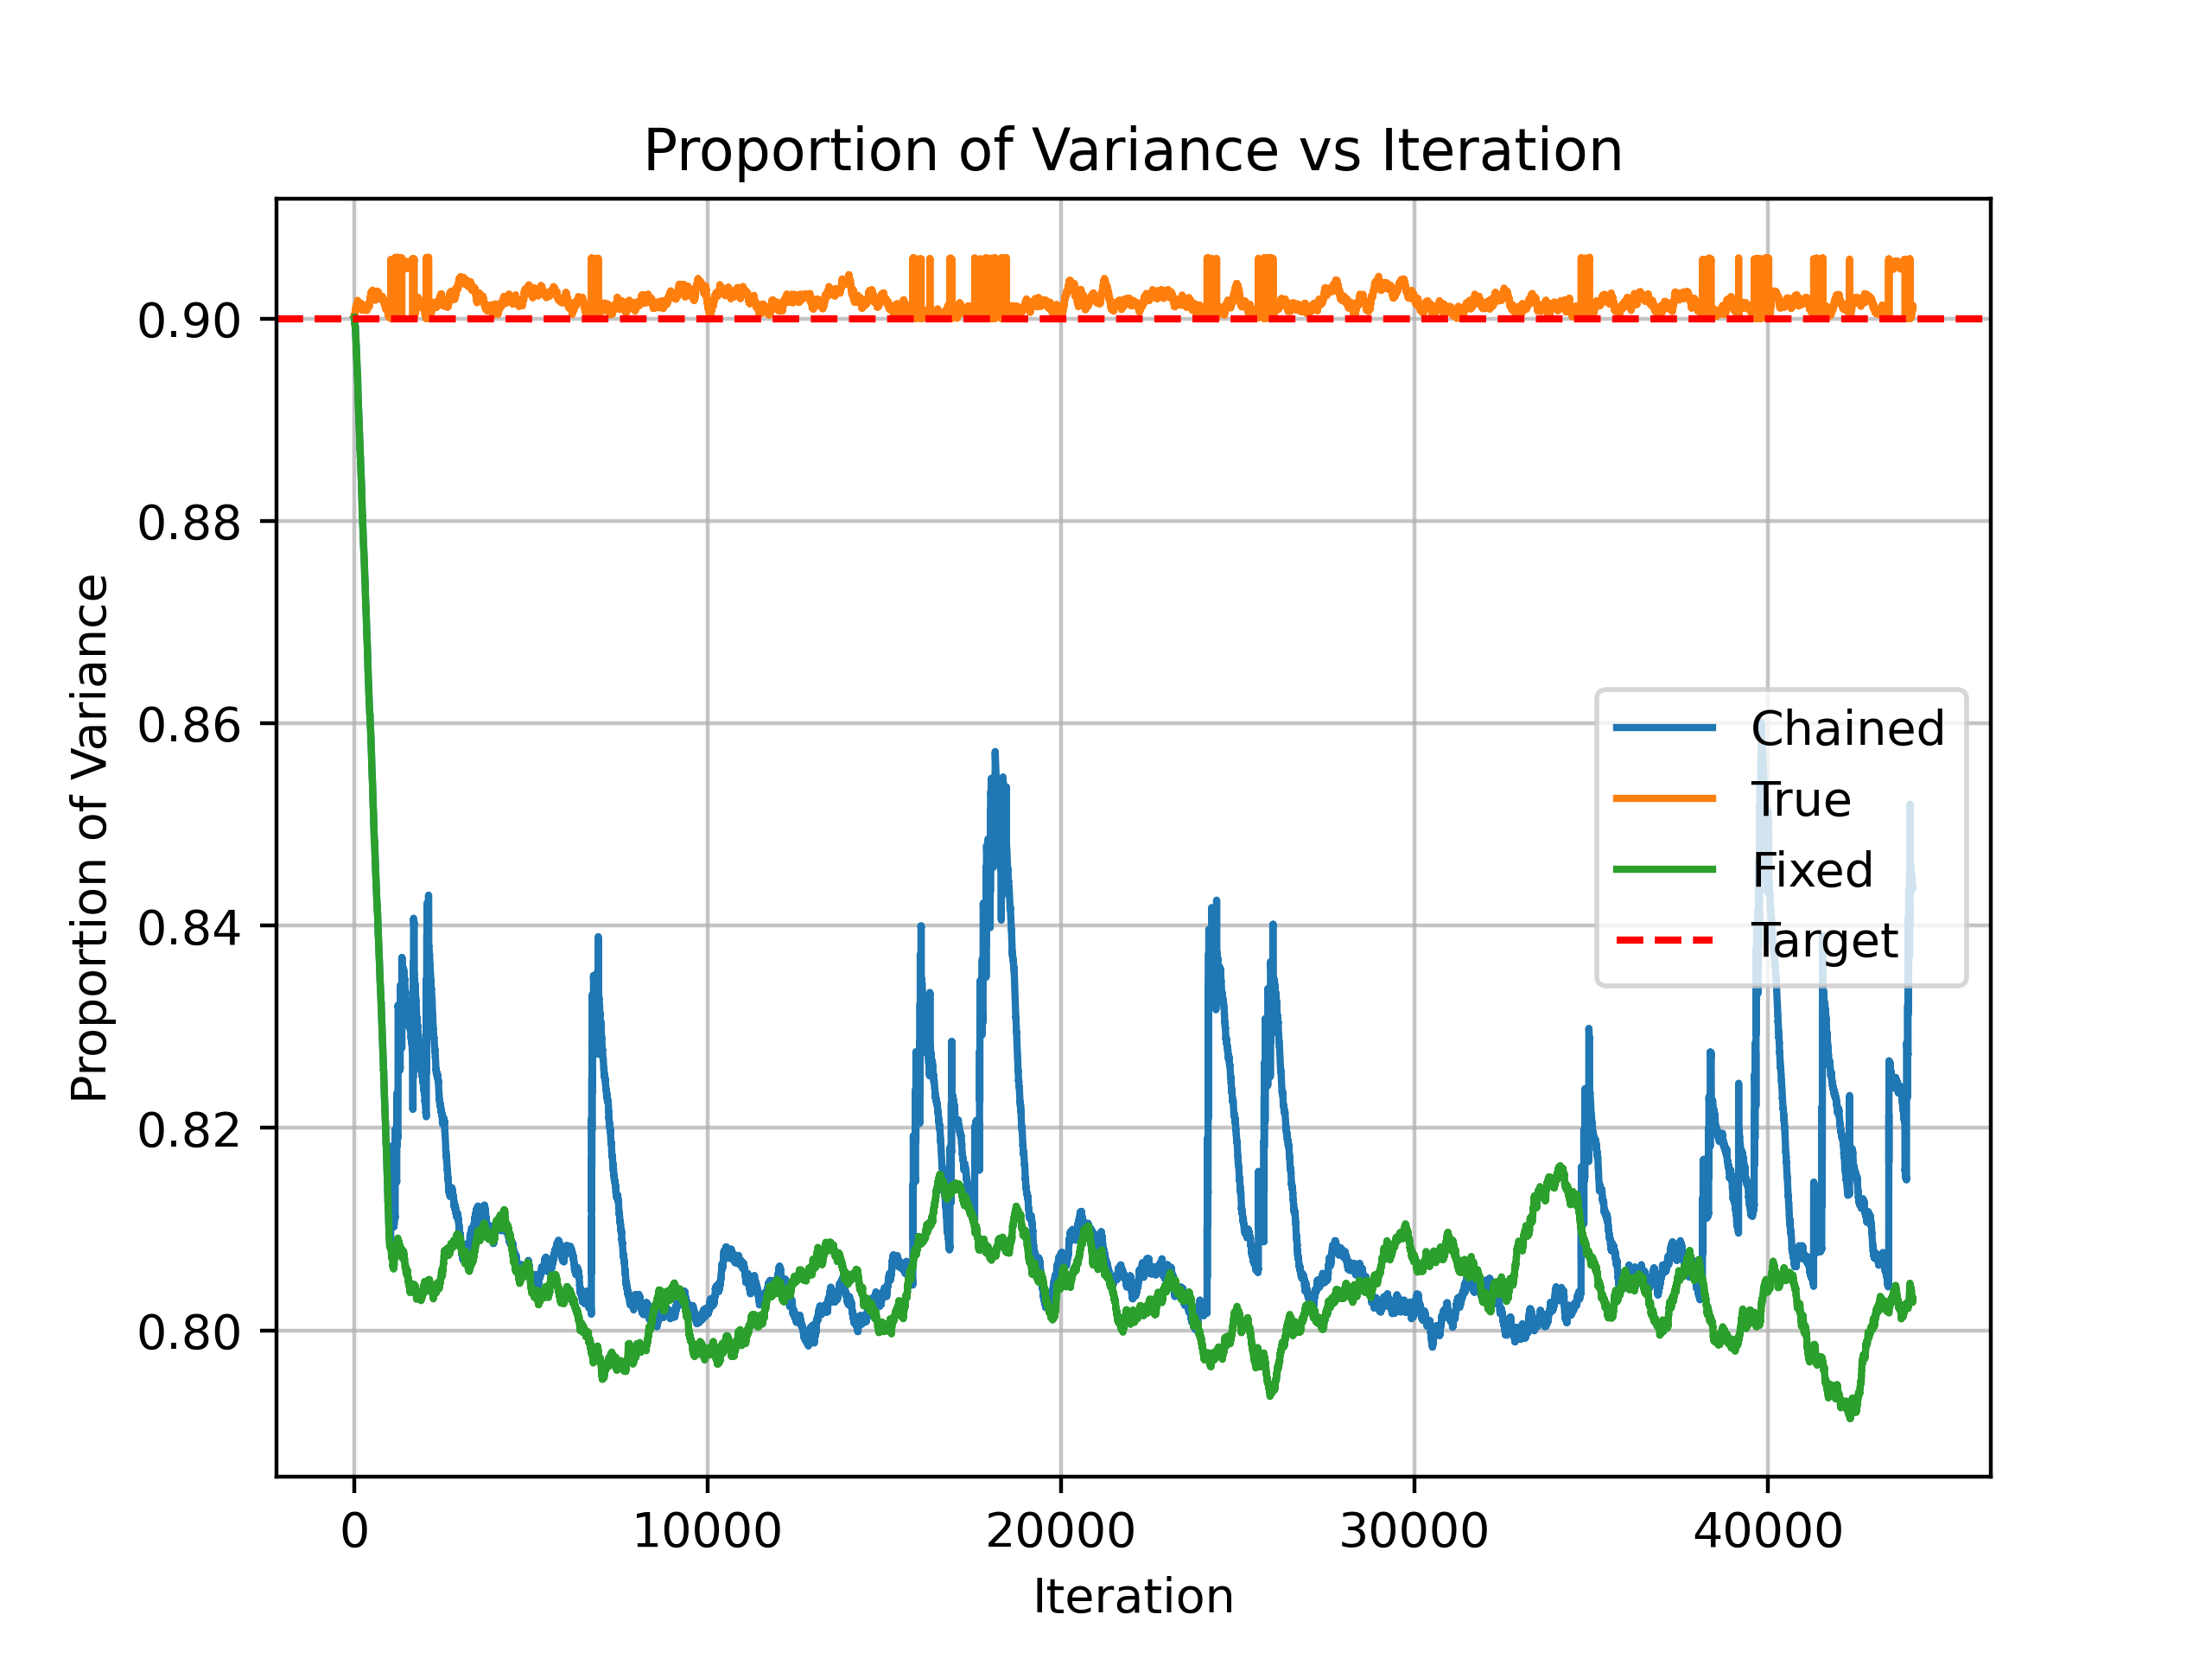
\includegraphics[width=0.8\textwidth]{figures/propvar.png}
    \caption{Proportion of variance retained by method.}
    \label{fig:propvar}
\end{figure}
We observe from Figure \ref{fig:propvar} that the Chained approach is generally more performant than with the fixed projection, however, it is not always better. Note that our projection chaining does not assume anything about the rotation structure; it just cares that the loadings are changing over time. One can entertain the idea that if a rotation structure is assumed, then all that is needed is to estimate the angle step in each plane, then in theory we circumvent the information loss issue. However, the rotation structure does not have an immediate real world application, so there is no grounds to even assume this when chaining projections.
\subsection{Static Kalman Filter}
Simulations have been largely done, but still need to produce the plots. Will provide:
\begin{itemize}
    \item Residual accuracy (based on a normalised version of $\mathrm{var}(\tilde{y})$) using the estimated $\bm{\beta}$, maximised over initial choices of $P,Q\in \{10^{-4}I,10^{-3}I, 10^{-2}I, 10^{-1}I\}$.
    \item Compare a few dimensions of $\beta$ vs. $\hat{\beta}$.
    \item Time performance.
\end{itemize}
\subsection{Dynamic Kalman Filter}
Have only run small scale tests so far. Will produce same plots/tables as above.
